%----------------------------------------------------------------------------
\chapter{Design}
\label{cha:design}
%----------------------------------------------------------------------------

Generating test cases from a specific model based on two step from the model-based testing process (see fourth step at Chapter~\ref{cha:modelbasedtesting}), namely the modelling and test case formalization (test selection criteria, test case specification) phases. These steps will be discussed one by one, considering the previously defined requirements. 

\section{Modeling language}
\label{sec:modelinglanguage}


\subsection{UML state machine}
\label{sub:umlstatemachine}

As the goal is to generate test cases from state machines, that having an UML state machine like semantics, investigating the UML standard \cite{omguml} can not be missed in this thesis.

UML state machines or UML state charts are improved versions of the mathematical concept of finite state automatons expressed with the OMG's Unified Modeling Language. The idea behind this notation is, that an entity or each of its sub-entities is always in exactly one of a number of possible states and where there are well-defined conditional transitions between these states. UML state charts introduce new features over traditional finite automatons such as hierarchically nested regions, orthogonal regions and actions. There are two kinds of state machine, which can be used to define behaviour of model elements and describe protocol usage.

\begin{figure}[htp]
\centering
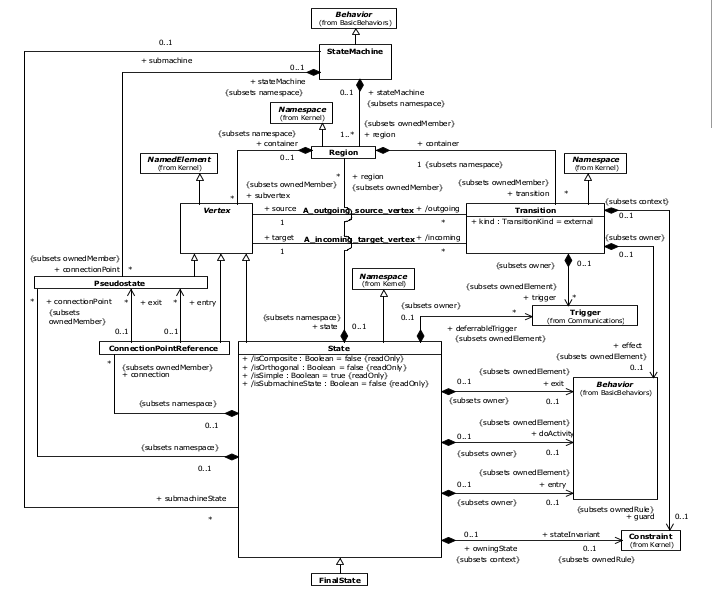
\includegraphics[scale=0.5]{figures/statemachine_metamodel}
\caption{Metamodel of UML state machine}
\label{fig:statemachine_metamodel}
\end{figure}

UML state machines are similar to traditional state machines, the main parts of them are the followings:

\begin{description}
	\item[States] are the phases of the system's history. For example if the history can be separated into two phases, then there are two states. 
	\item[Extended states] represents the complete condition of the system. This interpretation means usually states extended with system variables.
	\item[Transitions] happens when a state switched to another.
	\item[Actions] executed when an event dispatched and the system responds by performing them.
	\item[Events] can be everything, that happens with the system, and causes state change.
	\item[Guards] are boolean expressions described with extended state variables and event parameters. They can affect the system's behaviour by enabling or disabling transitions.
	\item[Hierarchically nested regions] means that if a system is in a substate then it is also in the same time in all the substate's superstates.
	\item[Orthogonal regions] are regions, which are in 'OR' relation.
\end{description}

% subsection umlstatemachine (end)

\subsection{PLC-HSM}
\label{sub:plchsm}

PLC-HSM is a modelling language intended to be a formal,
modular, hierarchical specification for describing PLC programs. It was created as part of a doctoral programme by Dániel Darvas of the Budapest University of Techology and Economics (BUTE) and the European Organization for Nuclear Research (CERN).

\begin{figure}[htp]
\centering
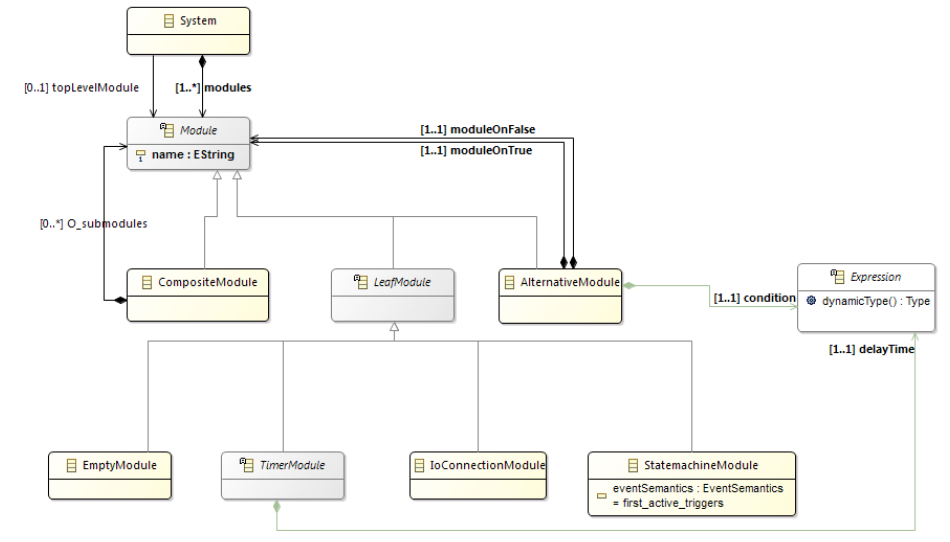
\includegraphics[scale=0.4]{figures/plchsm_modules}
\caption{Module structure of PLC-HSM}
\label{fig:plchsm_modules}
\end{figure}

The specification organized into modules (Figure~\ref{fig:plchsm_modules}), which are either represent a behaviour of concrete module (\texttt{LeafModule}) or they are composite modules containing a set of submodules (\texttt{CompositeModule}). There are four different module type:

\begin{itemize}
	\item \texttt{StatemachineModule} represents an UML-like state machine.
	\item \texttt{IoConnectionModule} defined by connections between input and output variables.
	\item \texttt{TimerModule} describes a PLC timer in the system.
	\item \texttt{EmptyModule} is a module without any state machine or IO connection.
\end{itemize}

From these module types we are interested especially in the state machine notation. As shown on Figure~\ref{fig:plchsm_statemachine} the metamodel is similar to UML state machine's metamodel described in the previous section.

\begin{figure}[htp]
\centering
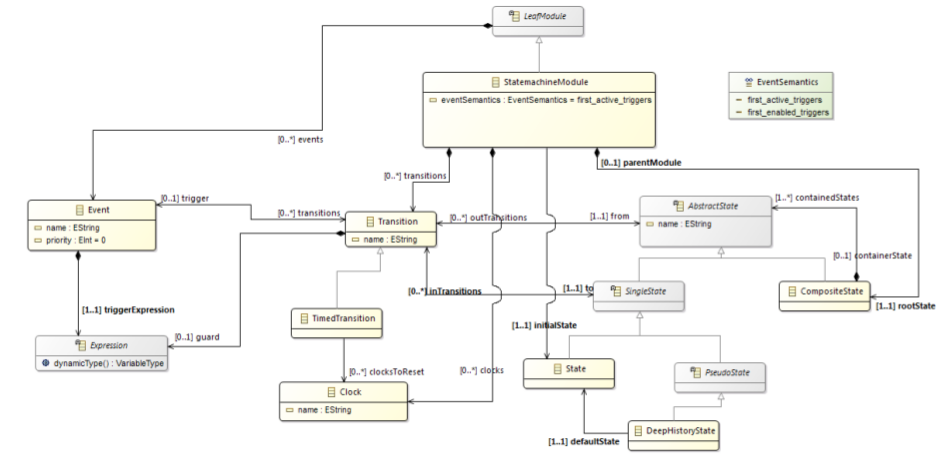
\includegraphics[scale=0.5]{figures/plchsm_statemachine}
\caption{Structure of \texttt{StatemachineModule}}
\label{fig:plchsm_statemachine}
\end{figure}

On the other hand PLC-HSM has some difference from the UML notation:

\begin{itemize}
	\item There is a root state, that recursively contains all of states.
	\item There are pseudo states (\texttt{DeepHistoryState}), which can save a state configuration for its container state.
	\item There are \texttt{TimedTransitions}, which are transitions having time-related conditions.
	\item With \texttt{Clocks} it is possible to define synchronous stopwatches, which can measure the elapsed time since last reset.
	\item Parallel regions are not allowed.
	\item Initial state can not be defined for composite states.
	\item At every moment, exactly one atomic state can be active. 
\end{itemize}

% subsection plchsm (end)

We can see, that PLC-HSM has some advantage over traditional UML modeling language:

\begin{itemize}
	\item UML language has only an informally given semantics.
	\item Tools having UML state machine creating capabilities are not standardised.
	\item PLC-HSM is rather a subset of the UML state machine language, and so it is more simple.
\end{itemize}

% section modelinglanguage (end)

\section{Test generation algorithms}
\label{sec:testgenerationalgorithms}

\subsection{Alloy}
\label{sub:alloy}

Alloy is a formal modeling language to define structures. Alloy can be utilised with a tool, called Alloy Analyzer to automate the verification process. The tool transforms problems into SAT formulas to solve them. The solver was inspired by model checkers, but it is implemented as a solver, performing verification within a bounded scope.

The strength of this tool allows us to define our test generation goals with the Alloy language to generate the test cases. The test cases need to guarantee state-based and transition-based coverages.

% subsection alloy (end)

% section testgenerationalgorithms (end)

% chapter design (end)